% Schematic of the Farhi--Neven QNN (hand-drawn TikZ, no data).
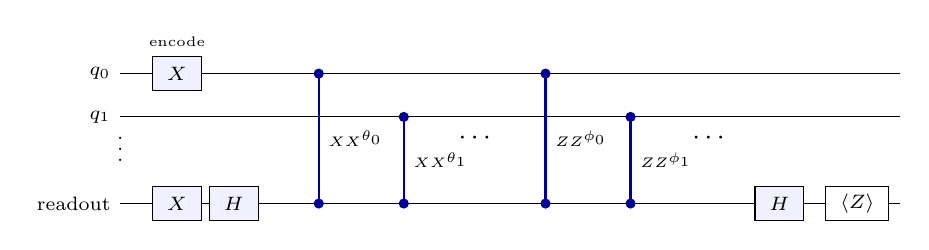
\begin{tikzpicture}[x=0.9cm,y=0.55cm,
  g/.style={draw,fill=blue!6,minimum width=0.62cm,minimum height=0.44cm,inner sep=1pt,font=\scriptsize},
  dot/.style={circle,fill=blue!60!black,inner sep=1.3pt}]
  \foreach \y/\n in {2/{$q_0$},1/{$q_1$}} \draw (0,\y) node[left,font=\scriptsize]{\n} -- (11,\y);
  \node[font=\scriptsize] at (0,0.45) {$\vdots$};
  \draw (0,-1) node[left,font=\scriptsize]{readout} -- (11,-1);
  \node[g] at (0.8,2) {$X$};
  \node[font=\tiny,above] at (0.8,2.4) {encode};
  \node[g] at (0.8,-1) {$X$}; \node[g] at (1.6,-1) {$H$};
  \foreach \x/\y/\l in {2.8/2/XX^{\theta_0},4.0/1/XX^{\theta_1},6.0/2/ZZ^{\phi_0},7.2/1/ZZ^{\phi_1}} {
    \draw[blue!60!black,thick] (\x,\y) -- (\x,-1);
    \node[dot] at (\x,\y) {}; \node[dot] at (\x,-1) {};
    \node[font=\tiny,right] at (\x,{(\y-1)/2}) {$\l$};
  }
  \node at (5.0,0.5) {$\cdots$}; \node at (8.3,0.5) {$\cdots$};
  \node[g] at (9.3,-1) {$H$};
  \node[g,fill=white,minimum width=0.8cm] at (10.4,-1) {$\langle Z\rangle$};
\end{tikzpicture}
